\documentclass[11pt]{article}
\usepackage{../../timestamp}
\usepackage{../../astro207}
\usepackage{../../markup}
\usepackage{../../fa21}
\usepackage{tikz}
\usetikzlibrary{calc,shapes.geometric,arrows,automata}
\usepackage{color,hyperref,listings,enumitem}
\usepackage{algorithm}
\usepackage{algpseudocode}
\usepackage{tkz-euclide}
\usepackage{pgfplots}
\usepackage{subcaption}
\usepackage{pdfpages}
\usepackage{bm}
\usepackage[american,siunitx]{circuitikz}
\lstset{basicstyle=\ttfamily}
\newcommand{\fillin}[1]{\underline{\hskip #1}}
\newcommand{\doublehrule}{\hrule \vskip 0.02in \hrule}
\newcommand*\circled[1]{\tikz[baseline=(char.base)]{
  \node[shape=circle,draw,inner sep=2pt] (char) {#1};}}
\usepackage{hyperref}
\hypersetup{
	colorlinks=true,
	linkcolor=black,
	urlcolor=blue
}

\begin{document}

\def\title{Problem Set 5}
% \config{hwnum}{1}
% \config{homework-due}{08/31/2018 23:59}
% \config{grades-due}{09/04/2018 23:59}

\newcommand{\qitem}{\qpart\item}

\renewcommand{\labelenumi}{(\arabic{enumi})} % change default enum format to (1)
\renewcommand{\theenumi}{(\arabic{enumi})} % fix reference format accordingly.
\renewcommand{\labelenumii}{\roman{enumii}.} % second level labels.
\renewcommand{\theenumii}{\roman{enumii}.}

\maketitle
\begin{qunlist}
\qns{Good Rovibrations}

\begin{enumerate}
\qitem{
	Assume we end in $n=0$.}
\work{
	\begin{align*}
		k_\text{center} &= \frac{\nu_\text{center}}{c}\\
		\nu_\text{center} &= ck_\text{center}\\
			&\approx 3(10^{10})\cdot 2145\\
			&\approx 6.4(10^{13}) \si{\hertz}\\
			&\approx 1\times\nu_{0,\text{CO}}
	\end{align*}
	where $\nu_{0,\text{CO}} \approx 6.7(10^{13}) \si{\hertz}$ is the natural frequency of CO's vibrational transition.}
\ans{
	\centering
	$|\Delta n| = 1$}

\qitem{
	\begin{itemize}
		\item Boltzmann statistics for populations in each $J$ state
		\item Line intensity $\propto$ $n_{J_\text{upper}}$
	\end{itemize}}
\work{
	\begin{align*}
	    \frac{n_{J+1}}{n_J} &= \frac{g_{J+1}}{g_J}e^{-\frac{E_{J+1} - E_J}{k_BT}}\\
			\text{where } E_{J+1} - E_J &= \frac{\hbar^2}{2I}\left[(J+1)(J+2) - J(J+1)\right]\\
			&= \frac{\hbar^2}{I}(J+1) \longleftarrow \begin{cases}
				I \approx \mu a_0^2\\
				\mu \equiv m_O \parallel m_C
					\end{cases}\\
	\end{align*}
	Sweeping $\frac{n_{J+1}}{n_J}$ with respect to $T$ and choosing $J_\text{infl}=7$ where $\frac{n_{J_\text{infl}}}{n_{J_\text{infl}-1}} > 1$ and $\frac{n_{J_\text{infl}+1}}{n_{J_\text{infl}}} < 1$ yields a rough temperature range
	\begin{figure}[H]
		\centering
		\textcolor{red}{INCLUDE}
		\label{fig:ratio_vs_temp}
	\end{figure}}
\ans{
	$$T\in [416, 526)\si{\kelvin}$$
}

\qitem{}
\work{
	Looking up the dipole moment $d_\text{CO} \approx 0.122 \text{ esu.}\si{\centi\meter}$ and calculating values relative to the Lyman-$\alpha$
	$$A_\text{CO} =  A_{\text{Ly}\alpha}\left(\frac{d_\text{CO}}{d_\text{H}}\right)^2\left(\frac{\omega_\text{CO}}{\omega_{\text{Ly}\alpha}}\right)^3$$
	with
	\begin{align*}
		\omega_\text{CO} &= \frac{(\Delta E)_{\substack{\Delta n=1\\\Delta J=\pm1}}}{\hbar}\\
			&= \omega_{0,\text{CO}} \pm \frac{\hbar}{I}J_\text{upper}
	\end{align*}
	\begin{figure}[H]
		\centering
		\textcolor{red}{INCLUDE}
		\label{fig:A_vs_J}
	\end{figure}}
\ans{
	\centering
	$A$ varies by more than 10\% over the range of $J$--enough to justify inclusion.}

\qitem{}
\work{
	\begin{align*}
		j_\nu &= \frac{h\nu}{4\pi}n_{J_\text{upper}}A_{21}
	\end{align*}
}
\ans{}

\qitem{\textcolor{white}{blep}}
\ans{
	A few things weren't accounted for:
	\begin{itemize}
		\item non-constant line profile function vs. frequency
		\item change and asymmetry in the moment of inertia (internuclear separation) with respect to $n$
	\end{itemize}}
\end{enumerate}
\end{qunlist}
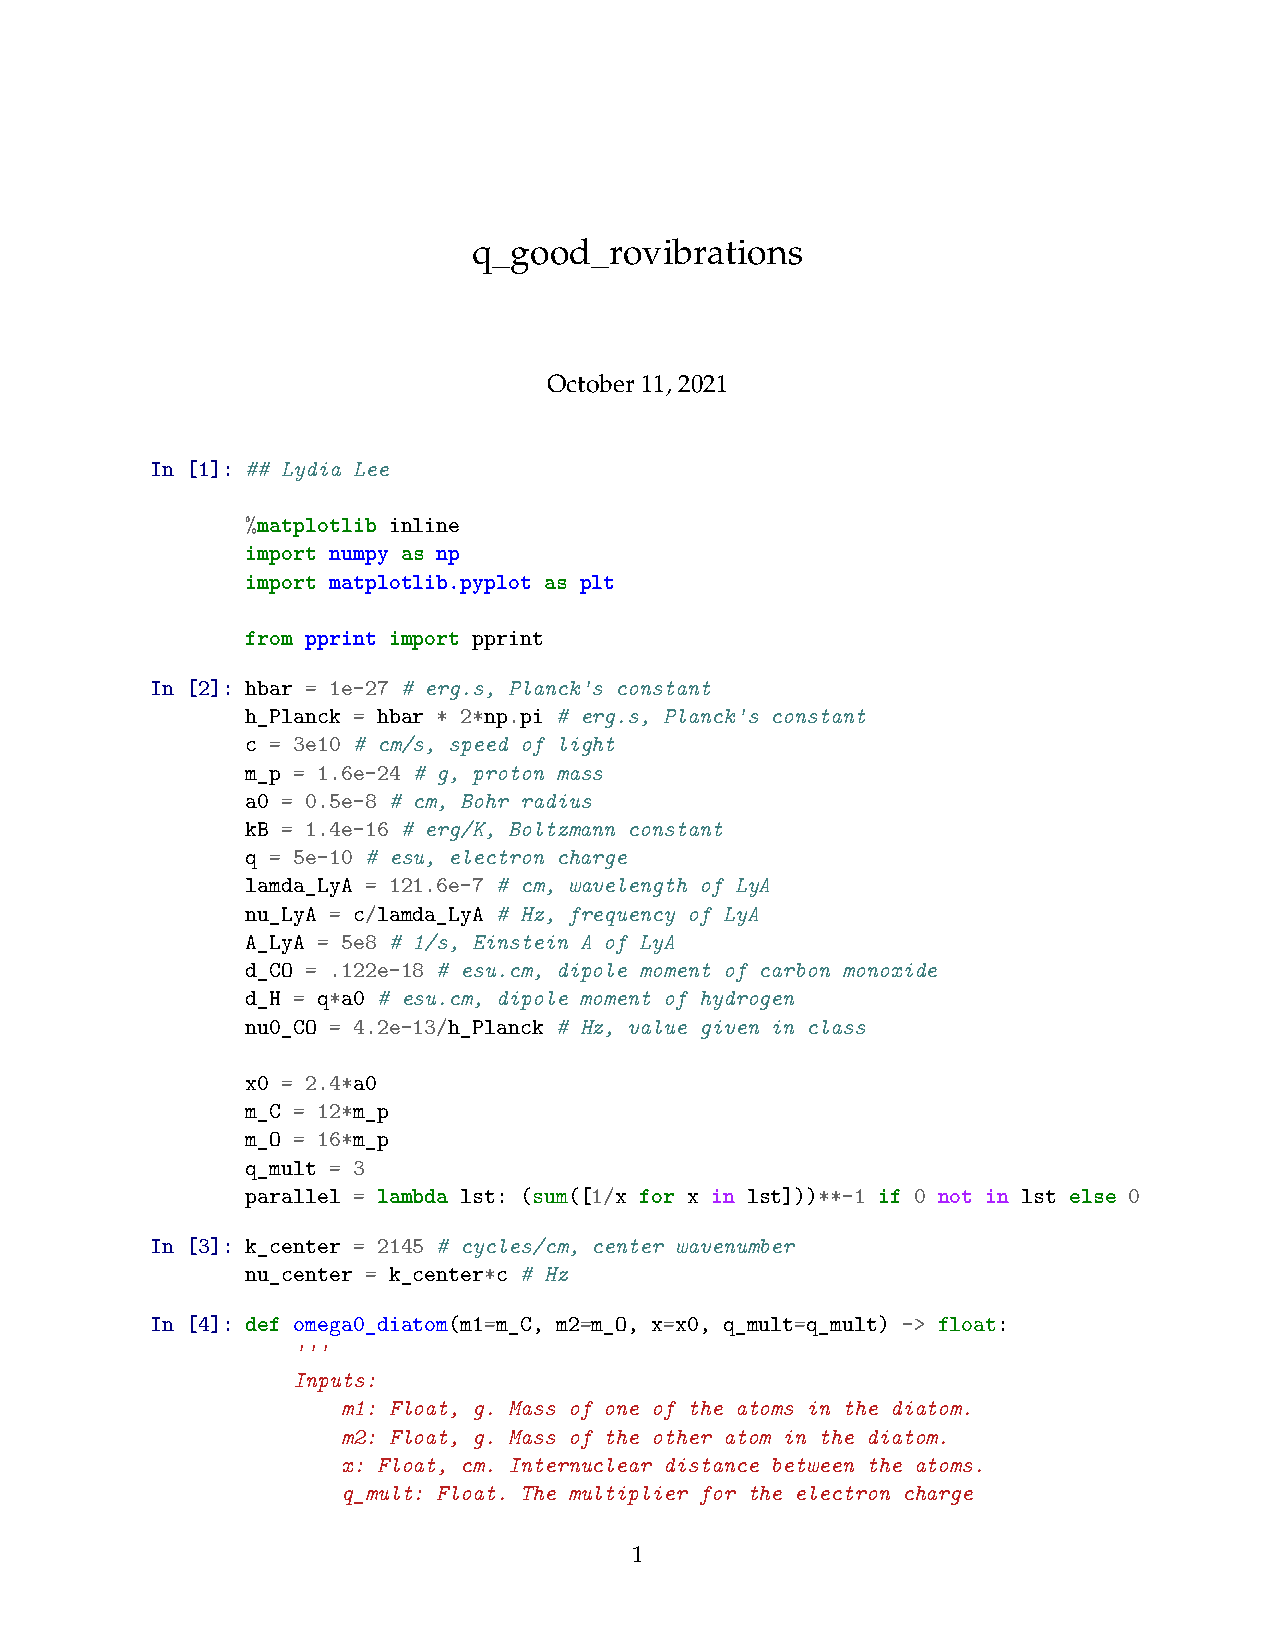
\includepdf[pages=-]{./questions/q_good_rovibrations_figs/q_good_rovibrations_ipynb.pdf}
\end{document}
